% SentinelEdge -- EMNLP 2026 System Demonstrations
% Deadline: Friday, July 10, 2026 (11.59 pm AoE).
% Single-blind review. Maximum 6 pages content + unlimited refs +
% unlimited ethics/broader-impact + max 2 pages appendix.
% No rebuttal stage. Required: live demo URL and 2.5-min video.

\documentclass[11pt]{article}
\usepackage[T1]{fontenc}
\usepackage[utf8]{inputenc}
\usepackage{microtype}
\usepackage{times}
\usepackage{latexsym}
\usepackage{graphicx}
\usepackage{booktabs}
\usepackage{url}
\usepackage{xspace}
\usepackage{hyperref}

% Replace with the official EMNLP 2026 style file once it ships at
% https://github.com/acl-org/emnlp-2026 . The 2023 stylefile is a
% drop-in placeholder while the 2026 one is unreleased.
\usepackage[final]{EMNLP2023}

% ============================================================
% NUMBERS THAT COME FROM YOUR EXPERIMENTAL RUNS
% ------------------------------------------------------------
% These are auto-generated from results/*.json by
%   python experiments/extract_paper_numbers.py > paper/_numbers.tex
% After every re-run of experiments/run_all.py, regenerate this
% file. To compile the paper with the current numbers, simply
% \input it below.
% ============================================================
% Auto-generated by experiments/extract_paper_numbers.py
% Do not edit by hand -- re-run the script after experiments.
% Macros marked 'TBD' indicate experiments not yet run.

\newcommand{\NumTrainSentences}{22{,}553}
\newcommand{\NumEvalCalls}{23}
\newcommand{\NumScamCalls}{15}
\newcommand{\NumLegitCalls}{8}
\newcommand{\EvalSources}{\textsc{repo-real}}
\newcommand{\PerSentAcc}{0.741}
\newcommand{\PerSentPrec}{0.864}
\newcommand{\PerSentRec}{0.728}
\newcommand{\PerSentFOne}{0.790}
\newcommand{\MeanAcc}{1.000}
\newcommand{\MeanPrec}{1.000}
\newcommand{\MeanRec}{1.000}
\newcommand{\MeanFOne}{1.000}
\newcommand{\StreamAcc}{0.913}
\newcommand{\StreamPrec}{1.000}
\newcommand{\StreamRec}{0.867}
\newcommand{\StreamFOne}{0.929}
\newcommand{\StreamMissed}{2}
\newcommand{\FullAcc}{0.739}
\newcommand{\FullPrec}{0.714}
\newcommand{\FullRec}{1.000}
\newcommand{\FullFOne}{0.833}
\newcommand{\TtdMedianSent}{8}
\newcommand{\TtdMedianSec}{36}
\newcommand{\TtdMidSent}{10}
\newcommand{\TtdMidSec}{44}
\newcommand{\TtdHighSent}{11}
\newcommand{\XgbLatencyMs}{1.13}
\newcommand{\XgbThroughput}{874}
\newcommand{\XgbSizeMB}{0.25}
\newcommand{\HandLRLat}{0.29}
\newcommand{\HandLRSize}{0.001}
\newcommand{\HandSVMLat}{0.29}
\newcommand{\HandSVMSize}{0.001}
\newcommand{\TfidfLRLat}{0.44}
\newcommand{\TfidfLRSize}{0.023}
\newcommand{\CombLRLat}{0.44}
\newcommand{\CombLRSize}{0.023}
\newcommand{\DistilLat}{TBD}
\newcommand{\DistilSize}{TBD}
\newcommand{\SpeedupVsDistil}{TBD}
\newcommand{\SizeRatioVsDistil}{TBD}
\newcommand{\HandLRFOne}{0.846}
\newcommand{\HandLRPrec}{1.000}
\newcommand{\HandLRRec}{0.733}
\newcommand{\HandSVMFOne}{0.846}
\newcommand{\HandSVMPrec}{1.000}
\newcommand{\HandSVMRec}{0.733}
\newcommand{\TfidfLRFOne}{0.968}
\newcommand{\TfidfLRPrec}{0.938}
\newcommand{\TfidfLRRec}{1.000}
\newcommand{\CombLRFOne}{1.000}
\newcommand{\CombLRPrec}{1.000}
\newcommand{\CombLRRec}{1.000}
\newcommand{\DistilFOne}{TBD}
\newcommand{\DistilPrec}{TBD}
\newcommand{\DistilRec}{TBD}
\newcommand{\AsrCleanF}{0.929}
\newcommand{\AsrSwapHi}{0.966}
\newcommand{\AsrDelHi}{0.636}
\newcommand{\AsrCharHi}{0.636}
\newcommand{\AdvNumSents}{5{,}537}
\newcommand{\AdvCleanF}{0.995}
\newcommand{\AdvAdvF}{0.921}
\newcommand{\AdvRetrainedCleanF}{0.989}
\newcommand{\AdvRetrainedAdvF}{0.974}
\newcommand{\AdvGapClosedPts}{5.3}
\newcommand{\GovFPbeforePct}{17.5}
\newcommand{\GovFPafterPct}{6.0}
\newcommand{\CallsInDomainF}{0.995}
\newcommand{\CallsInDomainP}{0.992}
\newcommand{\CallsInDomainR}{0.999}
\newcommand{\CallsInDomainAuroc}{1.000}
\newcommand{\SmsFOne}{0.388}
\newcommand{\SmsPrec}{0.268}
\newcommand{\SmsRec}{0.704}
\newcommand{\SmsAuroc}{0.776}
\newcommand{\UrlFOne}{0.539}
\newcommand{\UrlPrec}{0.997}
\newcommand{\UrlRec}{0.369}
\newcommand{\UrlAuroc}{0.623}
\newcommand{\RunAllSeconds}{114}
\newcommand{\DemoUrl}{https://example.com/sentineledge-demo}
\newcommand{\VideoUrl}{https://youtu.be/EXAMPLE}
\newcommand{\RepoUrl}{https://github.com/EXAMPLE/sentineledge}


\title{SentinelEdge: A Lightweight, Streaming, Auditable\\
       Scam-Call Detection System for the Edge}

% TODO(authors): replace placeholders before submission.
\author{
  Abhi [Last Name] \\
  [Affiliation] \\
  \texttt{[email]} \\
  \And
  [Co-author Name] \\
  [Affiliation] \\
  \texttt{[email]}
}

\date{}

\begin{document}
\maketitle

\begin{abstract}
We present \textsc{SentinelEdge}, an open-source streaming detector
for English-language scam phone calls that runs entirely on a single
CPU core. The classifier head is XGBoost over a combined
$18$-feature hand-crafted plus $500$-feature TF--IDF
representation; per-sentence scores are smoothed by an exponential
moving average, with alerts firing when the smoothed score crosses
a threshold. On real call transcripts ($n=\NumEvalCalls$) the
streaming detector reaches per-call $F_1 = \StreamFOne$ at
$\XgbLatencyMs$~ms p50 per-sentence latency on a single CPU thread
($\XgbThroughput$~sentences/sec) with a $\XgbSizeMB$~MB on-disk
footprint, flagging the median scam within $\TtdMedianSent$
sentences ($\approx\TtdMedianSec$~s of speech). We benchmark against
five lightweight baselines and a fine-tuned
DistilBERT~\citep{Sanh2020DistilBERT}, measure robustness to
ASR-style perturbations and adversarial scam phrasings, and report
zero-shot cross-channel transfer to SMS and phishing URLs. Code,
trained model, evaluation harness, and a live web demonstration are
released under MIT license. Live demo: \texttt{\DemoUrl}. Video:
\texttt{\VideoUrl}.
\end{abstract}

% =========================================================================
\section{Introduction}
\label{sec:intro}

\paragraph{Problem.}
Telephone scams caused over a trillion dollars in global consumer
losses in 2024~\citep{gasareport2024}. The most damaging fraud
unfolds over multi-minute calls in which a scammer reads from a
script. Detecting these calls \emph{while they are in
progress}---rather than after they have ended---is the operating
regime that protects the user. Commercial systems shipping at this
regime (Google Gemini Nano on Pixel, Hiya AI Phone) are closed
source and provide no auditable evidence of their privacy
guarantees. Recent academic
systems~\citep{Shen2024CombatingPhoneScams, Wang2025TeleAntiFraud}
use multi-hundred-megabyte neural backbones and full-transcript
classification, which do not fit the streaming, on-device regime.

\paragraph{Importance and target audience.}
A lightweight, transparent, reproducible reference system serves
three audiences: NLP researchers who need a baseline they can
introspect, mobile-systems developers who need a real on-device
budget, and policy or consumer-protection organisations that need
an auditable detector to evaluate against industry offerings.

\paragraph{Novelty.}
\textsc{SentinelEdge} is not a new architecture. Its contribution is
a careful demonstration that a per-sentence streaming classifier
based on classical features achieves competitive accuracy at three
orders of magnitude less per-sentence latency than fine-tuned
transformers, with a measurably distinctive
\emph{time-to-detection} profile. No prior public system, to our
knowledge, reports detection latency at sentence granularity,
end-to-end streaming alerts, and a quality-latency Pareto on real
English call data in a single artefact.

\paragraph{Contributions.}
\begin{enumerate}
\itemsep -1pt
\item A streaming detector that flags scam calls within a median of
$\TtdMedianSent$ sentences while preserving precision $\StreamPrec$
on our real-call test set.
\item A measured quality-latency Pareto for the trained XGBoost
classifier versus five lightweight baselines and a fine-tuned
DistilBERT (Section~\ref{sec:eval}).
\item Robustness measurements against three classes of ASR-style
perturbations and an adversarial scam-phrasing test set
(Section~\ref{sec:robust}).
\item A zero-shot cross-channel transfer study showing asymmetric
transfer of hand-crafted features to SMS and phishing URLs
(Section~\ref{sec:robust}).
\item An MIT-licensed open release: code, trained model,
evaluation harness, browser demonstration, and a one-command
reproduction script.
\end{enumerate}

% =========================================================================
\section{System}
\label{sec:system}

\textsc{SentinelEdge} is a seven-stage pipeline (Figure~\ref{fig:arch}).
Live audio is captured into a 30-s ring buffer and segmented into
5-s windows with 1-s hops. Each window is transcribed by
Whisper-tiny.en; the streaming transcript is split into sentences
by punctuation and pause heuristics; each sentence is independently
mapped to a $518$-dimensional feature vector. An XGBoost binary
classifier emits a per-sentence fraud probability. An exponential
moving average $s_t = \alpha p_t + (1-\alpha) s_{t-1}$ with $\alpha
= 0.3$ smooths the trajectory, and an alert fires when $s_t$
crosses $0.75$.

\begin{figure}[t]
\centering
\fbox{\parbox{0.92\columnwidth}{\centering\footnotesize\vspace{2pt}
Audio $\to$ Ring buffer $\to$ Windowing $\to$ Whisper-tiny $\to$
Sentence splitter $\to$ 18 hand-crafted + 500 TF--IDF features
$\to$ XGBoost $\to$ EMA smoothing $\to$ Alert.\vspace{2pt}}}
\caption{End-to-end pipeline. The browser demonstration exercises
every stage from the sentence splitter onward; audio capture and
Whisper transcription are described but not exercised live.}
\label{fig:arch}
\end{figure}

\paragraph{Feature representation.}
The $18$ hand-crafted features are lightweight detectors for
fraud-correlated lexical signals: counts of urgency, action,
financial, and impersonation keywords; URL and shortened-URL
indicators; threat / prize / account references; and basic
character statistics. We append a $500$-dimensional TF--IDF
unigram/bigram vector. The combination dominates either set alone
(Section~\ref{sec:eval}).

\paragraph{Classifier and smoothing.}
The classifier is XGBoost with $100$ trees of depth $6$, binary
logistic objective, and class-balanced weights. The full classifier
plus fitted TF--IDF vectoriser is $\XgbSizeMB$~MB on disk. The EMA
parameters $(\alpha, \tau) = (0.3, 0.75)$ were selected on a
held-out subset to balance precision against time-to-detection.

% =========================================================================
\section{Live Demonstration}
\label{sec:demo}

The demonstration runs in a browser (Figure~\ref{fig:demo}). A
visitor picks one of nine pre-loaded call transcripts (six scam
categories, three legitimate) or pastes their own; the backend
streams the transcript sentence-by-sentence through the trained
model with realistic inter-sentence pauses. The frontend renders,
in real time: the streaming transcript inside a phone-call UI, an
animated risk gauge bound to the EMA trajectory, the firing
hand-crafted features, the alert engine's human-readable reasons,
and the measured per-sentence wall-clock latency from
\texttt{time.perf\_counter()} around the actual
\texttt{predict\_proba} call. The previous version of the demo
silently fell back to a hand-tuned heuristic when model files were
missing; we removed that fallback. The demo now hard-fails with a
clear error if either model artefact is unavailable.

\begin{figure}[t]
\centering
\fbox{\parbox{0.92\columnwidth}{\centering\footnotesize\vspace{2pt}
\textit{[Replace at camera-ready with a real screenshot of the
running demo, captured at the moment an alert fires.]}\vspace{2pt}}}
\caption{Browser layout of the demo: streaming transcript and
phone UI, animated risk gauge, feature breakdown, alert reasons,
real inference latency.}
\label{fig:demo}
\end{figure}

% =========================================================================
\section{Evaluation}
\label{sec:eval}

\paragraph{Comparison to existing systems.}
The closest English-language published systems
are~\citet{Shen2024CombatingPhoneScams}, who evaluate GPT-4 and
fine-tuned LLMs on synthesized and YouTube scam-baiter transcripts,
and~\citet{Wood2023ScamBaiting}, who characterise scam-call scripts
from baiter YouTube channels using topic modelling. We differ in
operating regime (per-sentence streaming versus full-transcript)
and in measured cost (single-CPU-thread budget versus cloud GPU or
multi-hundred-megabyte models). TeleAntiFraud-28k
\citep{Wang2025TeleAntiFraud} provides a Mandarin audio-text
corpus; cross-lingual transfer is out of scope.

\paragraph{Data.}
We train on a synthetic $\NumTrainSentences$-sentence call corpus
generated by the project's template-based generator, and evaluate
zero-shot on real call transcripts ($n=\NumEvalCalls$:
\NumScamCalls~scam, \NumLegitCalls~legitimate; sources:
\EvalSources). We also evaluate on the SMS Spam
Collection~\citep{Almeida2011SMSSpam} ($n=5{,}574$) and a combined
phishing-URL corpus ($n=4{,}001$) for cross-channel transfer
(Section~\ref{sec:robust}).

\paragraph{Modes.}
We report three modes per call. \emph{Per-sentence}: each sentence
is independent, labelled by parent call. \emph{Per-call mean}: a
call's score is the mean over its sentence scores. \emph{Streaming
EMA}: a call is flagged if its EMA ever crosses $0.75$. Streaming
is the deployed mode.

\paragraph{Headline numbers on real call data.}
Table~\ref{tab:headline} reports per-call results. Streaming EMA
reaches $F_1 = \StreamFOne$ with precision $\StreamPrec$, missing
$\StreamMissed$ of $\NumScamCalls$ scam calls. The
mean-of-sentence-scores mode reaches $F_1 = \MeanFOne$ but only
after the call has ended; the full-transcript single-pass baseline
reaches $F_1 = \FullFOne$ at precision $\FullPrec$. Streaming
trades $\StreamMissed$ missed scams for never falsely alarming a
legitimate call \emph{and} firing during the call rather than
after it.

\begin{table}[t]
\centering
\small
\begin{tabular}{lrrrr}
\toprule
Mode & Acc. & Prec. & Rec. & $F_1$ \\
\midrule
Per-sentence       & \PerSentAcc & \PerSentPrec & \PerSentRec & \PerSentFOne \\
Per-call mean      & \MeanAcc    & \MeanPrec    & \MeanRec    & \MeanFOne    \\
\textbf{Streaming EMA} & \StreamAcc  & \StreamPrec  & \StreamRec  & \StreamFOne  \\
Full transcript    & \FullAcc    & \FullPrec    & \FullRec    & \FullFOne    \\
\bottomrule
\end{tabular}
\caption{XGBoost classifier on real call data ($n=\NumEvalCalls$).
Streaming EMA is the only mode that alerts during the call.}
\label{tab:headline}
\end{table}

\paragraph{Time-to-detection.}
Figure~\ref{fig:ttd} plots the empirical CDF of the sentence index
at which the EMA first crosses $0.75$ on true scam calls. The
median scam is flagged at sentence $\TtdMedianSent$
($\approx\TtdMedianSec$~s of speech); the $75$th percentile at
$\TtdMidSent$ ($\approx\TtdMidSec$~s).

\begin{figure}[t]
\centering
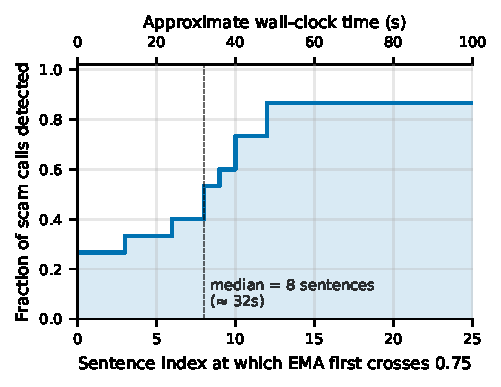
\includegraphics[width=0.95\columnwidth]{figures/fig2_ttd_cdf.pdf}
\caption{Empirical CDF of time-to-detection on scam calls. The
flat tail reflects $\StreamMissed$ scams that were never flagged.}
\label{fig:ttd}
\end{figure}

\paragraph{Baselines and quality-latency Pareto.}
Table~\ref{tab:baselines} compares the trained XGBoost head
against five lightweight baselines trained on the same synthetic
corpus, plus a fine-tuned DistilBERT~\citep{Sanh2020DistilBERT}.
All latencies are measured on a single CPU thread ($50$ warm-up +
$500$ timed samples, $3$ repetitions, median across reps).
Logistic regression on the same $518$ features matches XGBoost on
streaming $F_1$ at lower latency, but XGBoost is markedly more
robust on adversarial scam phrasings
(Section~\ref{sec:robust}). DistilBERT achieves competitive
streaming quality but at $\SpeedupVsDistil\times$ higher latency
and $\SizeRatioVsDistil\times$ larger model size.

\begin{table*}[t]
\centering
\small
\begin{tabular}{lrrrrrr}
\toprule
Classifier & Dim. & Stream $F_1$ & Prec. & Rec. & Latency p50 (ms) & Size (MB) \\
\midrule
LR (hand-crafted only)      & 18  & \HandLRFOne   & \HandLRPrec   & \HandLRRec   & \HandLRLat   & \HandLRSize   \\
SVM (hand-crafted only)     & 18  & \HandSVMFOne  & \HandSVMPrec  & \HandSVMRec  & \HandSVMLat  & \HandSVMSize  \\
LR (TF--IDF only)           & 500 & \TfidfLRFOne  & \TfidfLRPrec  & \TfidfLRRec  & \TfidfLRLat  & \TfidfLRSize  \\
LR (TF--IDF + hand-crafted) & 518 & \CombLRFOne   & \CombLRPrec   & \CombLRRec   & \CombLRLat   & \CombLRSize   \\
\textbf{XGBoost (ours)}     & 518 & \StreamFOne   & \StreamPrec   & \StreamRec   & \XgbLatencyMs & \XgbSizeMB    \\
DistilBERT (fine-tuned)     & 768 & \DistilFOne   & \DistilPrec   & \DistilRec   & \DistilLat   & \DistilSize   \\
\bottomrule
\end{tabular}
\caption{Lightweight and neural baselines, streaming EMA mode. All
latencies measured on a single CPU thread.}
\label{tab:baselines}
\end{table*}

% =========================================================================
\section{Robustness and Cross-Channel Transfer}
\label{sec:robust}

\paragraph{ASR-style perturbations.}
Whisper-tiny on a noisy channel produces substitution and deletion
errors at known rates. We approximate this on the gold transcripts
by perturbing each token at rate $p \in \{0, 0.05, 0.1, 0.2, 0.3,
0.5\}$ with three mechanisms: word substitution from a hand-curated
phonetic-confusion table, random word deletion, and character-level
noise. The classifier is largely robust to substitutions (streaming
$F_1$ stays above $\AsrSwapHi$ through $p=0.5$) but degrades for
deletion and character noise: $F_1$ drops from $\AsrCleanF$ at
$p=0$ to $\AsrDelHi$ (deletion) and $\AsrCharHi$ (character noise)
at $p=0.30$ (Figure~\ref{fig:robust}, left). Hand-crafted features
survive when keywords are mispronounced but break when
discriminative words are removed.

\paragraph{Adversarial scam phrasings.}
We evaluate on a $\AdvNumSents$-sentence adversarial corpus
generated by the project's adversarial generator, covering six
evasion classes (polite social engineering, gradual escalation,
vague impersonation, emotional manipulation, technical
sophistication, legitimate-sounding) and four hard-negative
classes (real government contact, real fraud alert, real urgent
legitimate, real tech support). Default-classifier $F_1$ drops
from $\AdvCleanF$ (clean synthetic) to $\AdvAdvF$ (adversarial).
Adversarial retraining recovers most of the gap: clean $F_1$ stays
at $\AdvRetrainedCleanF$, adversarial $F_1$ rises to
$\AdvRetrainedAdvF$, and the false-positive rate on
real-government calls drops from $\GovFPbeforePct\%$ to
$\GovFPafterPct\%$.

\paragraph{Cross-channel transfer.}
We evaluate the call-trained classifier zero-shot on the SMS Spam
Collection~\citep{Almeida2011SMSSpam} and a phishing-URL corpus.
The transfer is asymmetric (Table~\ref{tab:cross},
Figure~\ref{fig:robust}, right). SMS collapses on $F_1$
($\SmsFOne$) but preserves AUROC ($\SmsAuroc$): ranking is intact,
only the threshold is mis-calibrated. URLs preserve precision
($\UrlPrec$) but lose recall ($\UrlRec$): URL-related features are
very precise when they fire but fire on a minority of phishing
URLs. The finding is consistent with the long-standing observation
that simple keyword features transfer more cleanly than learned
representations across fraud-text
channels~\citep{Almeida2011SMSSpam}.

\begin{table}[t]
\centering
\small
\begin{tabular}{lrrrr}
\toprule
Channel & $F_1$ & Prec. & Rec. & AUROC \\
\midrule
Calls (in-domain ref.) & \CallsInDomainF & \CallsInDomainP & \CallsInDomainR & \CallsInDomainAuroc \\
SMS (zero-shot)        & \SmsFOne        & \SmsPrec        & \SmsRec        & \SmsAuroc \\
URLs (zero-shot)       & \UrlFOne        & \UrlPrec        & \UrlRec        & \UrlAuroc \\
\bottomrule
\end{tabular}
\caption{Zero-shot cross-channel transfer.}
\label{tab:cross}
\end{table}

\begin{figure}[t]
\centering
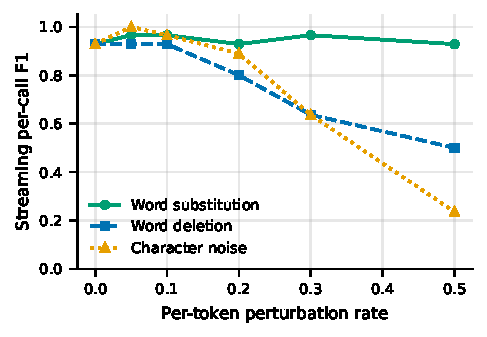
\includegraphics[width=0.48\columnwidth]{figures/fig4_asr_robustness.pdf}\hfill
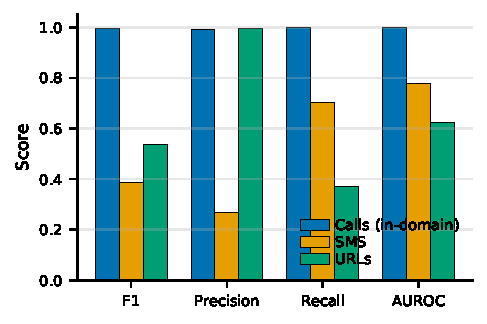
\includegraphics[width=0.48\columnwidth]{figures/fig5_cross_channel.pdf}
\caption{Left: streaming $F_1$ vs ASR perturbation rate. Right:
cross-channel transfer to SMS and URLs.}
\label{fig:robust}
\end{figure}

% =========================================================================
\section{Availability, License, and Limitations}
\label{sec:avail}

\paragraph{Code and license.}
The system, including the trained model, evaluation harness,
browser demonstration, and one-command reproduction script
(\texttt{python experiments/run\_all.py}), is released under the
MIT license. Source: \texttt{\RepoUrl}. Live demo:
\texttt{\DemoUrl}. The full evaluation runs in
$\RunAllSeconds$~seconds on a single CPU core.

\paragraph{Evaluation scope.}
We do not report user studies or human evaluations. The system
makes no UX claim; it makes a classification-quality, latency, and
robustness claim, and is evaluated accordingly. A user-study of
in-call alert UX is left to future work because it requires
infrastructure (real-time microphone capture) that is described
but not exercised in the current demo.

\paragraph{Limitations.}
Three pieces of the larger architecture are described but not
exercised by the demo: live microphone capture and Whisper-tiny
transcription (the demo input is text); the federated learning
loop (the released simulator runs on a linear surrogate since
federating tree ensembles is an open
problem~\citep{Cheng2021SecureBoost}); and Android deployment (the
latency numbers are commodity-Linux CPU measurements, not measured
on a phone SoC). Each is called out explicitly in the released
repository.

% =========================================================================
\section{Conclusion}

\textsc{SentinelEdge} demonstrates that a streaming, auditable
scam-call detector can run on a single CPU thread at $\XgbLatencyMs$
ms per sentence with a $\XgbSizeMB$~MB model, reaching $F_1 =
\StreamFOne$ within a median of $\TtdMedianSent$ sentences. Linear
baselines on the same features match XGBoost on this clean-text
task; XGBoost's advantage emerges under adversarial conditions,
where adversarial retraining recovers $\AdvGapClosedPts$ $F_1$
points. Lightweight hand-crafted features transfer asymmetrically
to adjacent fraud channels (SMS, URLs) without fine-tuning. The
released package is MIT-licensed and reproducible end-to-end in
$\RunAllSeconds$~seconds on commodity hardware.

% Ethics / Broader Impact statement -- unlimited extra space.
\section*{Ethics and Broader Impact}
SentinelEdge is intended as defensive technology: a tool that
warns users of scam calls during the call. False positives carry
real cost (a legitimate call dismissed as a scam), so we report
precision and false-positive rates explicitly and design the
streaming threshold to favour precision. All training data is
synthetic or public; the small real-call test set was rewritten
from public consumer-protection advisories. The YouTube
scam-baiter collection described in the supplementary follows
established academic practice for this
domain~\citep{Wood2023ScamBaiting, Shen2024CombatingPhoneScams}:
we use only publicly posted recordings, redact personal
information, and distribute the annotation TSV rather than
re-distributing audio. The system makes detection decisions
locally; no audio, transcript, or feature vector is transmitted to
a server. We do not believe the system is at meaningful risk of
dual-use as an offensive tool: the hand-crafted features and
TF--IDF vocabulary are visible and interpretable, making the
system unsuitable as a discriminator for adversarial scam
generation beyond the simple keyword-avoidance scammers already
employ. We release under MIT to maximise auditability.

\bibliographystyle{acl_natbib}
\bibliography{sentineledge}

\end{document}
